\begin{frame}{SL deep Interpolation vs classical interpolation}
    For $nt=100$ and different values of $nx$ we have:\\
    \textbf{1st Order Interpolation degree}
    \begin{figure}
        \centering
        
        \begin{subfigure}{0.2\textwidth}
            \centering
            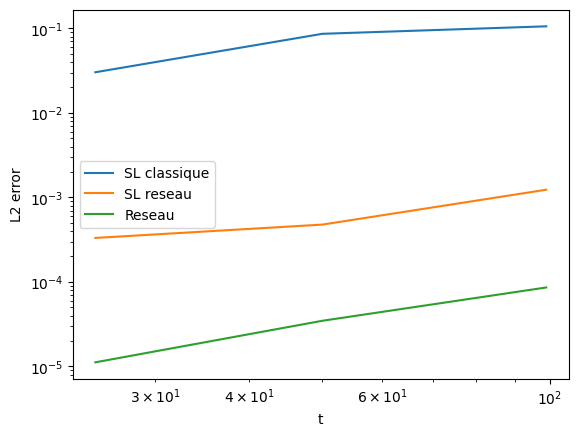
\includegraphics[width=\textwidth]{images/i110.png}
            \caption{nx=10}
        \end{subfigure}
        \begin{subfigure}{0.2\textwidth}
            \centering
            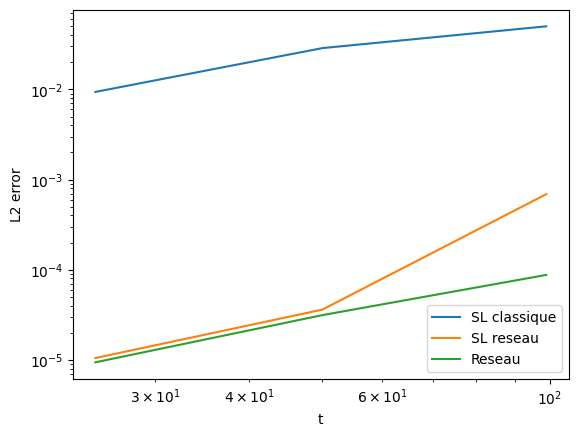
\includegraphics[width=\textwidth]{images/i120.png}
            \caption{nx=20}
        \end{subfigure}
        \begin{subfigure}{0.2\textwidth}
            \centering
            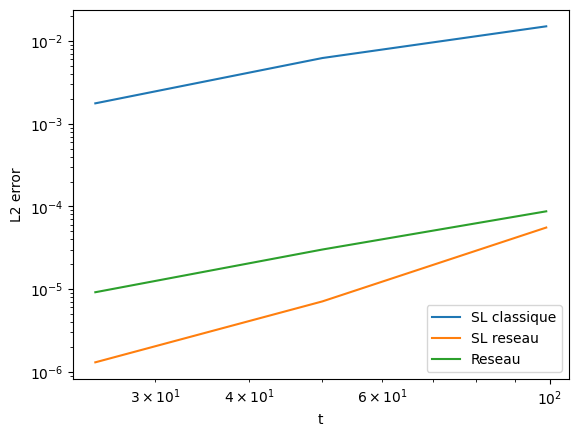
\includegraphics[width=\textwidth]{images/i1.png}
            \caption{nx=40}
        \end{subfigure}
    
    \end{figure}

    \textbf{3rd Order Interpolation degree}
    \begin{figure}
        \centering
        
        \begin{subfigure}{0.2\textwidth}
            \centering
            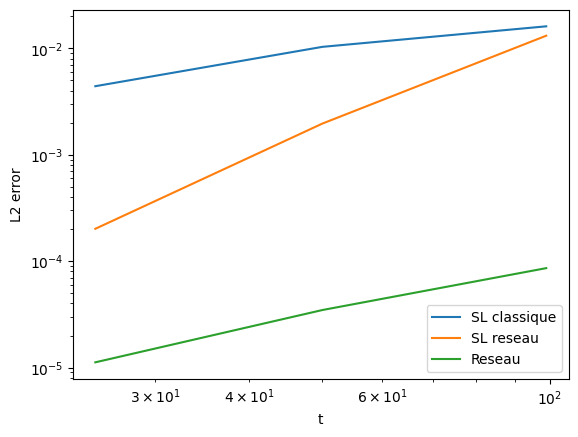
\includegraphics[width=\textwidth]{images/i310.png}
            \caption{nx=10}
        \end{subfigure}
        \begin{subfigure}{0.2\textwidth}
            \centering
            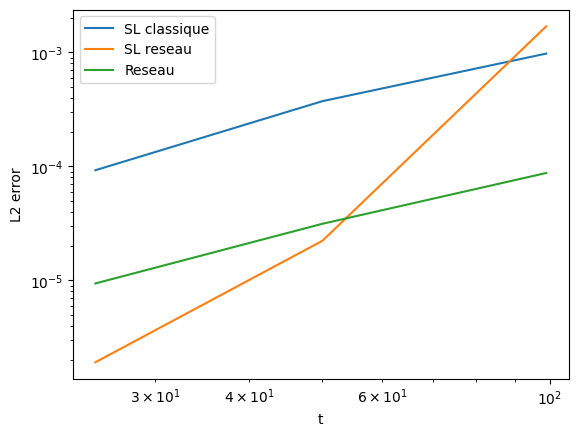
\includegraphics[width=\textwidth]{images/i320.png}
            \caption{nx=20}
        \end{subfigure}
        \begin{subfigure}{0.2\textwidth}
            \centering
            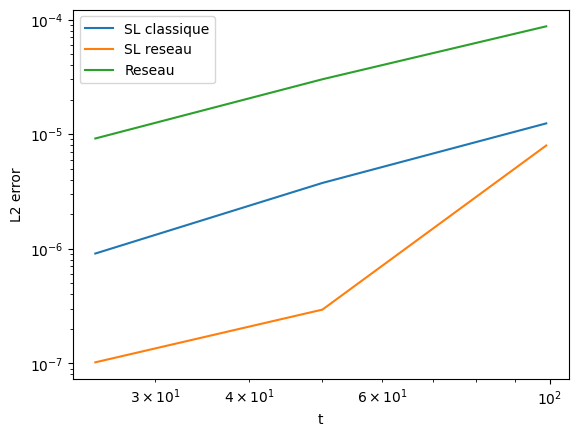
\includegraphics[width=\textwidth]{images/i3.png}
            \caption{nx=40}
        \end{subfigure}
    
    \end{figure}
   
    

\end{frame}